\chapter{Tools}
\label{chap:tools}
\setstretch{1.5}
In this chapter an overview of the used robot, sensors, tools and software is given. Each section contains a brief description and hardware components include a specification list. Data sheets will be attached in the appendix.
\section{Hardware and Software}
\label{sec: hwsw}
\subsection{Fanuc CR-35iA}
\label{subsec:fanuc}
The Fanuc CR-35iA \cite{Fanuc} is one of the strongest collaborative robots currently available on the market. It can lift up to 35kg and has a maximum reach of 1.8m. The robot is designed to collaborate with humans on heavy and repetitive jobs in industries like automotive, packaging, distribution and metalworking. The robot body is coated with a soft rubber skin to prevent injuries and is ISO 10218-1:2011 certified. The certification specifies requirements and guidelines for the inherent safe design, protective measures and information for use of industrial robots. The robot is equipped with a Fanuc R-30iB controller. Figure \ref{fig:fanuc_human} shows the Fanuc CR-35iA besides the author for a size comparison.


\begin{figure}[H]
	\centering\includegraphics[scale=0.2]{images/robo_human.jpeg}			
	\caption{Fanuc CR-35iA robot side-by-side with a human for size comparison.}
	\label{fig:fanuc_human}
\end{figure}

%https://www.fanuc.eu/ch/en/robots/robot-filter-page/collaborative-robots/collaborative-cr35ia
%https://www.iso.org/standard/51330.html


\subsection{Asus Xtion PRO LIVE}
\label{subsec:asus}
The Asus Xtion PRO LIVE \cite{Asus} (figure \ref{fig:asus}) camera uses infrared sensors, adaptive depth detection technology and color image sensing to capture the user's real time image and movements. It is designed for gesture and whole body detection and has a set of predefined functions to support these tasks. The camera uses USB 2.0 Interface. The distance of use is between 0.8m and 3.5m. This camera was used since it was already available multiple times in the same version, the specifications meet the requirements and it was already used in similar projects.

\begin{figure}[H]
	\centering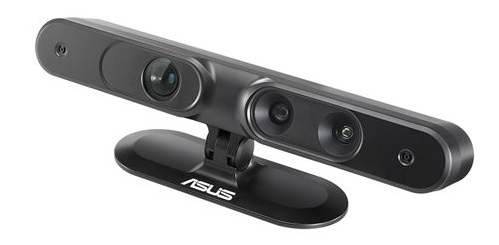
\includegraphics[scale=0.5]{images/Asus_Xtion_PRO_Live.jpg}			
	\caption{Asus Xtion PRO LIVE camera}
	\label{fig:asus}
\end{figure}


%http://xtionprolive.com/asus-3d-depth-camera/asus-xtion-pro-live

\subsection{Roboguide}
\label{subsec:roboguide}
Roboguide is an offline programming software for Fanuc robots. It allows the user to create programs for the robot and simulate its workspace in 3D without the physical need and expense of a prototype workspace setup. Two different types of programs can be used with the robot. Teach pendant or TP programs are mostly used for robot motions and calling other programs. TP programs can either be written on the teach pendant or within the Roboguide software. KAREL programs are used when the TP programs reach their limits. KAREL is a language very similar to Pascal. It features strongly typed variables, constants, custom types, functions and provides all sorts of built-ins for things which can't be done with TP. Karel is a compiled language, therefor the source must be translated from a KAREL file (.kl) into p-code (.pc) which is typically done in Roboguide. Roboguide and the two programming languages were used to establish a socket communication with an external C++ program. Figure \ref{fig:roboguide} shows the simulated workspace in Roboguide.

\begin{figure}[H]
	\centering\includegraphics[scale=0.3]{images/roboguide.png}			
	\caption{Simulated workspace environment in Fanuc Roboguide.}
	\label{fig:roboguide}
\end{figure}

\subsection{CloudCompare}
\label{subsec:cloudcomp}
CloudCompare is a 3D point cloud processing open source software. It has been originally designed to perform comparison between two dense 3D point clouds or between a point cloud and a triangular mesh. It relies on a specific octree data structure dedicated to this task. CloudCompare has been extended to a more generic point cloud processing software, including many advanced algorithms like registration, resampling and interactive or automatic segmentation. In this project, CloudCompare is used for the camera calibration process.

\begin{figure}[H]
	\centering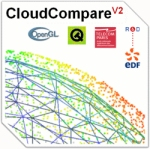
\includegraphics[scale=1]{images/cc_logo_v2_small.jpg}		
	\caption{CloudCompare logo.}
\end{figure}


\section{Libraries and Algorithms}
\label{sec:libalg}


\subsection{Point Cloud Library}
\label{subsec:pcl}
The Point Cloud Library (PCL) is a stand-alone, large scale, open project for 2D/3D image and point cloud processing. It is released under the  3-clause BSD license and thus free for commercial and research use. The PCL framework contains numerous state-of the art algorithms including filtering, surface reconstruction, registration, model fitting and segmentation. In this project, PCL is used to process the sensor data into point clouds, including filtering and transforming.

\begin{figure}[H]
	\centering
\includegraphics[scale=0.7]{images/pcl.png}			
	\caption{Point Cloud Library Logo.}
\end{figure}


\subsection{Octomap library}
\label{subsec:octomap} 
The Octomap library implements a 3D occupancy grid mapping approach, providing data structures and mapping algorithms in C++ particularly suited for robotics.  The map implementation is based on the octree data structure and is designed to provide a full 3D model with information about occupied, free and unknown cells. Information or new sensor readings can be added at any time and the extent of the map does not have to be known in advance. It is released under the  3-clause BSD license and thus free for commercial and research use.

